% =====================================================================
%  Introduction to Deep Learning — Class 27
%  Topic (course plan): Recurrent Neural Network
%  Subtopic (course plan): Encoder-decoder Seq-to-Seq
%  Sources (course plan): Jurafsky & Martin Ch. 13 (Ch. 14 in the
%    August 2026 draft: "RNNs and LSTMs"; Ch. 13 is now "Machine
%    Translation" and is used for beam search), Goodfellow Ch. 10
%
%  Class 26 built the simple recurrent network and trained it through
%  time.  This class asks what a recurrent network can do when the
%  output is itself a sequence of a different length: read one
%  sequence into a context, then write another from it.  The object
%  is the conditional language model p(y | x); the recurrent cell g is
%  a black box today and is opened in Class 28.
%
%  Order: the RNN language model in three equations; the task; the
%  encoder-decoder and its context; training by teacher forcing; the
%  bottleneck and the attention that removes it; decoding.
%
%  Three results are stated in neither textbook; the C variant is this
%  deck with those three removed.  See _shared/PLAN_Classes26_27_28_29.md.
%
%  Compile:  xelatex main.tex   (run twice)
% =====================================================================
\documentclass[aspectratio=169, 11pt]{beamer}

\usetheme{metropoliscustom}

\usepackage{graphicx}
\DeclareGraphicsExtensions{.pdf,.png,.jpg}
\graphicspath{{figs_official/}{Class27_Encoder_Decoder_Seq2Seq/A_Textbook_Figures/figs_official/}}
\usepackage{amsmath, amssymb}
\usepackage{bm}
\usepackage{tikz}
\usetikzlibrary{arrows.meta, positioning, calc, decorations.pathreplacing,
                shapes.geometric, fit, backgrounds}
\tcbuselibrary{skins}

\definecolor{shc}{HTML}{341651}
\definecolor{tealc}{HTML}{1C7293}
\definecolor{dpc}{HTML}{800000}
\definecolor{accc}{HTML}{B8860B}

% ---- theorem environments -------------------------------------------
\setbeamertemplate{theorems}[numbered]
\usepackage{remreset}
\makeatletter\@removefromreset{theorem}{section}\makeatother
\renewcommand{\thetheorem}{\arabic{theorem}}
\newtheorem{lemmax}[theorem]{Lemma}
\newtheorem{propx}[theorem]{Proposition}
\newtheorem{corx}[theorem]{Corollary}
\newtheorem{defx}[theorem]{Definition}
\newtheorem{thmx}[theorem]{Theorem}

\newcommand{\bridge}[1]{%
  {\scriptsize\itshape\color{mcMuted} #1\par}\vspace{0.35em}}

\newcommand{\srcline}[1]{%
  \par\vspace{0.25em}%
  {\scriptsize\color{mcMuted}\hfill #1\par}}

\newcommand{\figsource}[1]{{\scriptsize\color{mcMuted} #1}}
\newcommand{\figcap}[2][0.90]{%
  \begin{center}\begin{minipage}{#1\textwidth}\centering
    {\scriptsize\color{mcMuted} #2}
  \end{minipage}\end{center}}

\newcommand{\bos}{\langle s\rangle}
\newcommand{\eos}{\langle/s\rangle}

% =====================================================================
\title{Recurrent Neural Networks}
\subtitle{Encoder--Decoder: Sequence to Sequence}
\author{Introduction to Deep Learning \ \textperiodcentered\ Class 27}
\institute{}
\date{}

\footleft{Introduction to Deep Learning}
\footright{Encoder--Decoder}
\titlelogos{}

\begin{document}

\maketitle

\begin{frame}{Outline}
  \tableofcontents
\end{frame}

% =====================================================================
\section{From Reading to Writing}
% =====================================================================

\begin{frame}{Where we are coming from}
  \vspace{-0.3em}
  {\scriptsize
  \renewcommand{\arraystretch}{1.3}
  \begin{tabular}{@{}l@{\hspace{1.2em}}l@{}}
    \textbf{Class 26: the recurrent network} & \textbf{what it gave us}\\
    one cell, applied at every step & a reader for sequences of any length\\
    a state $\mathbf{h}_t$ carried from step to step & a memory of everything read so far\\
    $\mathbf{W}$ reads, $\mathbf{U}$ remembers, $\mathbf{V}$ answers & one answer per step, from the state\\
    back-propagation through time & the loss at any step reaches every earlier weight\\
  \end{tabular}}
  \vspace{0.4em}

  {\footnotesize
  \begin{itemize}\itemsep0.2em
    \item Every answer that network could give was tied to its reading:
          a label \alert{for each} token, one label \alert{for the whole}
          sequence, or the \alert{next} token after the ones read
    \item Today's task is different in kind: the answer is a
          \alert{new sequence} --- with its own length, its own order, and
          no token-by-token correspondence to the input
    \item The instinct carries over --- the same cell, the same state ---
          but the network will have to \alert{read first and write
          afterwards}, which needs two of them
  \end{itemize}}
  \srcline{Class 26; Jurafsky \& Martin (2026), \S14.7; Goodfellow et al.\ (2016), \S10.4.}
\end{frame}

\begin{frame}{The problem: one sequence into another}
  \vspace{0.05em}
  {\footnotesize
  \begin{itemize}\itemsep0.25em
    \item The running example, from Jurafsky \& Martin:
          \emph{the green witch arrived} $\longrightarrow$ \emph{lleg\'o la bruja verde}
    \item Four words in, four out --- but look at what moved: \emph{arrived}
          is last in English and \emph{lleg\'o} \alert{first} in Spanish;
          \emph{green witch} becomes \emph{bruja verde}, adjective after
          noun. No word sits where its translation sits
    \item Lengths differ too (\emph{I am hungry}: three words; \emph{tengo
          hambre}: two). Translation, summarising, answering a question,
          speech to text: all \alert{a sequence in, a different sequence out}
  \end{itemize}}
  \vspace{0.1em}
  \begin{redhighlight}
    The output cannot be produced token by token as the input is read:
    the first output word may depend on the last input word.
  \end{redhighlight}
  \srcline{Jurafsky \& Martin (2026), \S14.7, \S13.1; Goodfellow et al.\ (2016), \S10.4.}
\end{frame}

\begin{frame}{Why the tools we have fall short}
  \vspace{-0.1em}
  {\scriptsize
  \renewcommand{\arraystretch}{1.3}
  \begin{tabular}{@{}l@{\hspace{1.0em}}l@{\hspace{1.0em}}l@{}}
    \textbf{Class 26's reader as \ldots} & \textbf{what it produces} & \textbf{why it cannot translate}\\
    a tagger & one output per input, same position & \emph{lleg\'o} would have to come out at \emph{the}\\
    a classifier & one output for the whole input & a translation is not one label\\
    a language model & the next word, from the words before & no source to translate; it only continues\\
    a window & an output from a few nearby inputs & cannot see the last word when writing the first\\
  \end{tabular}}
  \vspace{0.4em}

  {\footnotesize
  \begin{itemize}\itemsep0.2em
    \item The tagger is closest and fails on exactly the point of the
          example: its outputs are \alert{aligned} with its inputs
    \item The language model is the right kind of machine --- it
          \alert{writes} any length, one word at a time --- but from nothing
          but its own previous words
    \item So the missing piece is not a new cell: it is a way to hand the
          language model \alert{the whole source} before it writes a word
  \end{itemize}}
  \srcline{Jurafsky \& Martin (2026), \S14.3, \S14.7; Class 26.}
\end{frame}

\begin{frame}{The idea: read everything, then write}
  \vspace{0.05em}
  {\footnotesize
  \begin{itemize}\itemsep0.28em
    \item How a person translates: read the sentence \alert{to the end},
          form an understanding, then write in the target language's own
          order. Nobody writes \emph{lleg\'o} before reading \emph{arrived}
    \item The equipment: \alert{two} recurrent networks of Class 26. The
          first \alert{reads} the source into its state --- the
          \alert{encoder}; its last state is the ``understanding'', one
          vector, the \alert{context}
    \item The second is a language model that \alert{writes}, primed with
          the context instead of nothing --- the \alert{decoder}: one word
          at a time, each fed back, until an end symbol
    \item Nothing inside either cell changes; only the wiring does. The
          class is that wiring, its training, what is wrong with one
          context vector, and how the decoder picks its words
  \end{itemize}}
  \vspace{0.1em}
  \begin{redhighlight}
    An encoder--decoder is a reader whose final memory becomes the
    starting memory of a writer.
  \end{redhighlight}
  \srcline{Jurafsky \& Martin (2026), \S14.7; Goodfellow et al.\ (2016), \S10.4; Cho et al.\ (2014); Sutskever et al.\ (2014).}
\end{frame}

\begin{frame}{Notation for today}
  \vspace{0.2em}
  {\footnotesize
  \renewcommand{\arraystretch}{1.28}
  \begin{columns}[T, onlytextwidth]
    \begin{column}{0.49\textwidth}
      \begin{tabular}{@{}l@{\hspace{1.3em}}l@{}}
        $\mathbf{x}_{1:n}$, $\mathbf{y}_{1:m}$ & source and target sequences\\
        $\mathbf{e}_t = \mathbf{E}\mathbf{x}_t$ & the embedding of token $t$\\
        $\mathbf{h}^e_t$, $\mathbf{h}^d_t$ & encoder and decoder states\\
        $\mathbf{W}, \mathbf{U}, \mathbf{V}$ & input, recurrent, output weights\\
      \end{tabular}
    \end{column}
    \begin{column}{0.49\textwidth}
      \begin{tabular}{@{}l@{\hspace{1.3em}}l@{}}
        $g(\cdot)$ & the recurrent cell, a black box today\\
        $\mathbf{c}$, $\mathbf{c}_i$ & the context: fixed, or per step\\
        $\alpha_{ij}$ & attention on source $j$ at target step $i$\\
        $\bos$, $\eos$ & start and end symbols\\
      \end{tabular}
    \end{column}
  \end{columns}}
  \vspace{0.45em}

  \begin{itemize}\itemsep0.22em
    \item Jurafsky writes $\mathbf{h}_t = g(\mathbf{U}\mathbf{h}_{t-1} + \mathbf{W}\mathbf{x}_t)$;
          Goodfellow writes the same with $\mathbf{U}$ and $\mathbf{W}$
          \alert{swapped} and time as a superscript, $\mathbf{h}^{(t)}$.
          This block follows Jurafsky's letters with time as a subscript
    \item The August 2026 draft numbers the RNN chapter 14, not 13;
          citations here follow that draft
  \end{itemize}
  \srcline{Jurafsky \& Martin (2026), Eqs.~14.1--14.3; Goodfellow et al.\ (2016), Eqs.~10.8--10.11.}
\end{frame}

% =====================================================================
\section{The Writer: a Language Model}
% =====================================================================

\begin{frame}{The recurrent language model, in three lines}
  \vspace{-0.45em}
  \begin{defx}[RNN language model]\label{th:lm}
    \small
    At step $t$, with $\mathbf{x}_t$ the one-hot of the current word,
    \[
      \mathbf{e}_t = \mathbf{E}\mathbf{x}_t, \qquad
      \mathbf{h}_t = g(\mathbf{U}\mathbf{h}_{t-1} + \mathbf{W}\mathbf{e}_t), \qquad
      \hat{\mathbf{y}}_t = \mathrm{softmax}(\mathbf{V}\mathbf{h}_t),
    \]
    and $\hat{\mathbf{y}}_t[k] = P(w_{t+1} = k \mid w_1, \dots, w_t)$.
  \end{defx}
  \vspace{-0.1em}
  {\footnotesize
  \begin{itemize}\itemsep0.2em
    \item Class 26's three jobs, with the answer fixed: $\mathbf{W}$
          \alert{reads} the word, $\mathbf{U}$ \alert{remembers} the words
          before it, $\mathbf{V}$ \alert{answers} ``which word comes next?''
          with a distribution over the vocabulary
    \item On \emph{The flights the airline was canceling}, the state still
          carries \emph{flights}, so the answer can be \emph{were}. The cell
          $g$ stays a black box (Class 28); training on text is Class 29.
          Today the model is a \alert{writer}
  \end{itemize}}
  \srcline{Jurafsky \& Martin (2026), Eqs.~14.4--14.7, Fig.~14.5; Class 26; Mikolov et al.\ (2010).}
\end{frame}

\begin{frame}{Generating, one token at a time}
  \begin{center}
    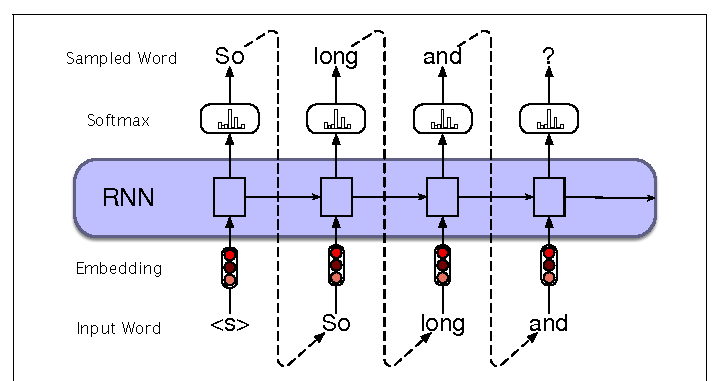
\includegraphics[height=0.50\textheight]{J14_9}
  \end{center}
  \vspace{-0.5em}
  {\tiny\color{mcMuted}
  Autoregressive generation with an RNN language model: start from
  $\bos$; the softmax gives a distribution over the next word; sample one
  (\emph{So}); feed its embedding back as the next input; sample again;
  stop at $\eos$ or a length limit. Every word is conditioned on the words
  the model itself chose. Every application today primes this loop with
  something richer than $\bos$: the source.
  \hfill Jurafsky \& Martin (2026), Fig.~14.9, \S14.3.3; Shannon (1951).\par}
\end{frame}
\begin{frame}{The probability of a whole sequence}
  \vspace{-0.45em}
  \begin{thmx}[Chain rule of sequences]\label{th:chain}
    \small
    For any distribution over sequences $\mathbf{y} = y_1, \dots, y_m$,
    conditioned on anything $\mathbf{x}$,
    \[
      p(\mathbf{y} \mid \mathbf{x}) = \prod_{t=1}^{m} p(y_t \mid y_1, \dots, y_{t-1}, \mathbf{x}).
    \]
    An identity, not a modelling assumption.
  \end{thmx}
  \vspace{-0.25em}
  {\footnotesize
  \begin{itemize}\itemsep0.12em
    \item \focus{1}{Proof. $p(y_1, y_2 \mid \mathbf{x}) = p(y_1 \mid \mathbf{x})\, p(y_2 \mid y_1, \mathbf{x})$
          by the definition of conditional probability; induct on $m$.
          \hfill $\square$}
    \item \focus{2}{The recurrent model parameterises each factor by one
          softmax with the prefix carried in $\mathbf{h}_{t-1}$: its one
          assumption is that a fixed-size state can carry the prefix.}
    \item \focus{3}{So a generated sequence's probability is the product
          of the next-token probabilities it chose.}
  \end{itemize}}
  \vspace{-0.45em}
  \srcline{Jurafsky \& Martin (2026), Eqs.~14.8--14.9, 14.28; Goodfellow (2016), Eq.~10.31.}
\end{frame}

% =====================================================================
\section{The Encoder--Decoder}
% =====================================================================

\begin{frame}{One change turns a language model into a translator}
  \vspace{-0.1em}
  {\footnotesize
  \begin{itemize}\itemsep0.30em
    \item Take the writer of the last section and give it a longer text
          to continue: the source, a separator, then the target:
          \[
            \text{the \ green \ witch \ arrived \ } \bos \text{ \ lleg\'o \ la \ bruja \ verde \ } \eos
          \]
    \item Run the language model over it. During \emph{the green witch
          arrived} its predictions are ignored --- it is only
          \alert{reading}, filling its state. From $\bos$ on, its next-word
          distribution is \alert{writing}, and every word it writes is
          conditioned on the source through that state
    \item That is the whole idea, and it already translates. What follows
          is giving the two halves names, drawing it, training it, and
          then fixing what is wrong with it
  \end{itemize}}
  \vspace{0.2em}
  \begin{redhighlight}
    An encoder--decoder is a conditional language model:
    $p(\mathbf{y} \mid \mathbf{x})$ with the source read first.
  \end{redhighlight}
  \srcline{Jurafsky \& Martin (2026), \S14.7, Eq.~14.31, Fig.~14.17.}
\end{frame}
\begin{frame}{The three parts}
  \vspace{-0.45em}
  \begin{defx}[Encoder--decoder network]\label{th:encdec}
    \small
    An \alert{encoder} reads $\mathbf{x}_{1:n}$ into states $\mathbf{h}^e_{1:n}$.
    A \alert{context} $\mathbf{c} = f(\mathbf{h}^e_{1:n})$ conveys the source to
    the decoder. A \alert{decoder} reads $\mathbf{c}$ and generates
    $\mathbf{h}^d_{1:m}$, hence $\mathbf{y}_{1:m}$, of any length. Either half
    may be any sequence architecture; here both are RNNs.
  \end{defx}
  \vspace{-0.35em}
  \begin{center}
  \begin{tikzpicture}[>=Stealth, font=\scriptsize, x=1cm, y=1cm,
      enc/.style={rounded corners=3pt, draw=shc, fill=shc!10, line width=1.0pt,
                  minimum width=3.4cm, minimum height=0.6cm},
      dec/.style={rounded corners=3pt, draw=dpc, fill=dpc!10, line width=1.0pt,
                  minimum width=3.4cm, minimum height=0.6cm},
      ctx/.style={rounded corners=3pt, draw=tealc, fill=tealc!12, line width=1.0pt,
                  minimum width=1.5cm, minimum height=0.55cm},
      ar/.style={->, line width=1.0pt}]
    \node[enc] (E) at (0,0) {Encoder};
    \node[ctx] (C) at (3.3,0.35) {Context $\mathbf{c}$};
    \node[dec] (D) at (6.6,0.7) {Decoder};
    \foreach \i/\l in {-1.3/{$x_1$}, -0.45/{$x_2$}, 0.4/{$\cdots$}, 1.3/{$x_n$}}{
      \draw[ar] ({\i},-0.85) node[below]{\l} -- ({\i},-0.3);}
    \foreach \i/\l in {5.3/{$y_1$}, 6.15/{$y_2$}, 7.0/{$\cdots$}, 7.9/{$y_m$}}{
      \draw[ar,dpc] ({\i},1.0) -- ({\i},1.5) node[above]{\l};}
    \draw[ar, shc] (E.east) -- (C.west);
    \draw[ar, tealc] (C.east) -- (D.west);
  \end{tikzpicture}
  \end{center}
  \vspace{-0.6em}
  \srcline{Jurafsky \& Martin (2026), \S14.7, Fig.~14.16; Goodfellow (2016), \S10.4; Cho et al.\ (2014); Sutskever et al.\ (2014).}
\end{frame}

\begin{frame}{Two ways to hand over a vector: as an extra input}
  \begin{center}
    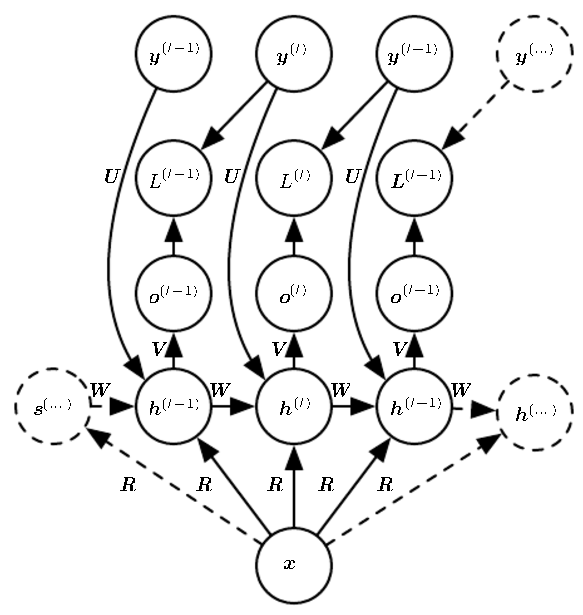
\includegraphics[height=0.56\textheight]{G10_9}
  \end{center}
  \vspace{-0.5em}
  {\tiny\color{mcMuted}
  Goodfellow's first way: a single fixed vector $x$ is fed as an extra
  input to every step of the recurrence through its own matrix $R$,
  while the sequence input at each step is the previous output; the
  network maps one vector to a sequence, and the vector's influence is
  renewed at every step. (His $W$ is the recurrent matrix, our $\mathbf{U}$.)
  \hfill Goodfellow et al.\ (2016), Fig.~10.9, \S10.2.4.\par}
\end{frame}

\begin{frame}{Two ways to hand over a vector: as the first state}
  \begin{center}
    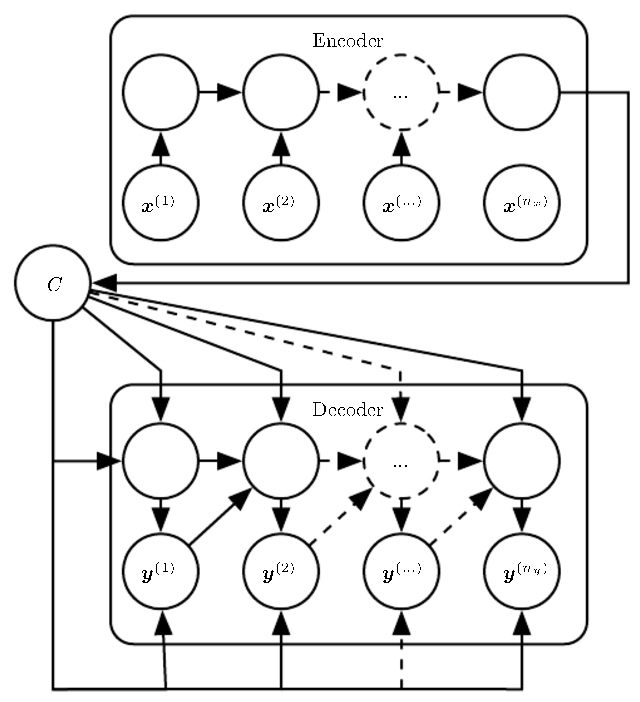
\includegraphics[height=0.58\textheight]{G10_12}
  \end{center}
  \vspace{-0.5em}
  {\tiny\color{mcMuted}
  Goodfellow's second way, the encoder--decoder itself: an encoder RNN
  reads $x^{(1)} \ldots x^{(n_x)}$ and emits a context $C$, usually its
  final state; a decoder RNN starts from $C$ and generates
  $y^{(1)} \ldots y^{(n_y)}$. The lengths $n_x$ and $n_y$ can differ.
  Jurafsky's Eq.~14.32 uses both ways at once.
  \hfill Goodfellow et al.\ (2016), Fig.~10.12, \S10.4.\par}
\end{frame}
\begin{frame}{The equations}
  \vspace{-0.3em}
  \begin{propx}[The basic RNN encoder--decoder]\label{th:eqs}
    \small
    With $g$ the recurrent cell and $\hat{\mathbf{y}}_{t-1}$ the embedding of
    the previous output,
    \[
      \mathbf{c} = \mathbf{h}^e_n, \qquad
      \mathbf{h}^d_0 = \mathbf{c}, \qquad
      \mathbf{h}^d_t = g(\hat{\mathbf{y}}_{t-1}, \mathbf{h}^d_{t-1}, \mathbf{c}), \qquad
      \hat{\mathbf{y}}_t = \mathrm{softmax}(\mathbf{V}\mathbf{h}^d_t).
    \]
  \end{propx}
  \vspace{0.05em}
  {\footnotesize
  \begin{itemize}\itemsep0.22em
    \item Two ways to hand over the context, and the equations use both:
          as the decoder's \alert{initial state} $\mathbf{h}^d_0$, and as an
          \alert{extra input at every step}, so its influence does not
          wane as the output grows
    \item The two previous drawings, combined: Goodfellow's extra input
          at every step (Fig.~10.9) and his first state (Fig.~10.12);
          Jurafsky's Eq.~14.32 is the sum of the two
    \item The encoder's own outputs are never used; in practice it is a
          stacked, bidirectional RNN (Class 26) and $\mathbf{h}^e_n$ is the top
          layer's last state
  \end{itemize}}
  \srcline{Jurafsky \& Martin (2026), Eqs.~14.32--14.33, Fig.~14.18; Goodfellow et al.\ (2016), \S10.2.4, Eq.~10.35.}
\end{frame}

\begin{frame}{The whole model on the example}
  \begin{center}
    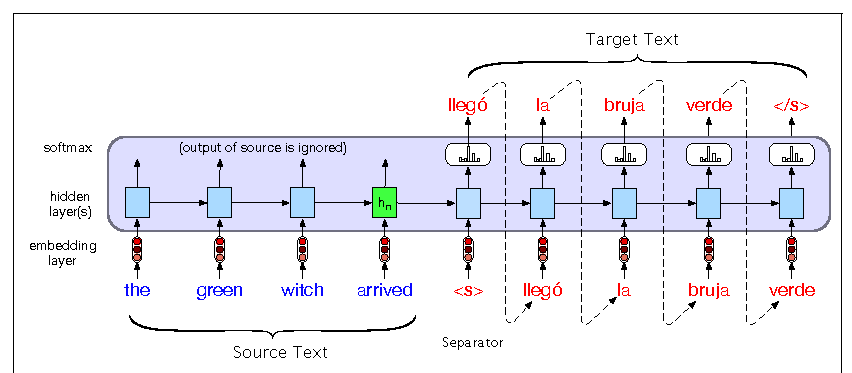
\includegraphics[width=0.92\linewidth]{J14_17}
  \end{center}
  \vspace{-0.5em}
  {\tiny\color{mcMuted}
  Translating the example at inference time: source and target
  concatenated with a separator, one network run over both; the outputs
  of the source steps are ignored; the last source state (green)
  conditions the target steps; each output word is the next input.
  \hfill Jurafsky \& Martin (2026), Fig.~14.17, \S14.7.\par}
\end{frame}

\begin{frame}{The encoder--decoder, unrolled}
  \begin{center}
    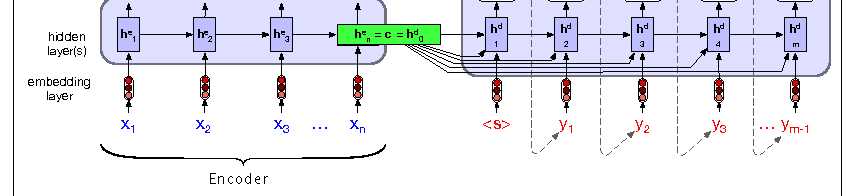
\includegraphics[width=0.98\linewidth]{J14_18}
  \end{center}
  \vspace{-0.5em}
  {\tiny\color{mcMuted}
  The same model with the two halves named: the encoder's final state is
  the context $\mathbf{c}$ and the decoder's first state $\mathbf{h}^d_0$; the
  context also enters every decoder step; the decoder reads $\bos$ and
  then its own previous output.
  \hfill Jurafsky \& Martin (2026), Fig.~14.18, Eqs.~14.32--14.33.\par}
\end{frame}

% =====================================================================
\section{Training}
% =====================================================================

\begin{frame}{Teacher forcing}
  \vspace{-0.55em}
  \begin{thmx}[Teacher forcing is maximum likelihood]\label{th:tf}
    \small
    Feed the decoder the \emph{gold} token $y_{t-1}$ at every step,
    not its own output, and sum the cross-entropy of each gold token:
    \[
      L(\mathbf{x}, \mathbf{y}) = -\sum_{t=1}^{m} \log \hat{\mathbf{y}}_t[y_t]
                           = -\log p(\mathbf{y} \mid \mathbf{x}).
    \]
    Minimising it maximises the likelihood of the target.
  \end{thmx}
  \vspace{-0.1em}
  {\footnotesize
  \begin{itemize}\itemsep0.16em
    \item \focus{1}{Proof. With gold inputs, step $t$'s softmax is the
          factor $p(y_t \mid y_{<t}, \mathbf{x})$ of Theorem~\ref{th:chain};
          the sum of the logs is the log of the product. \hfill $\square$}
    \item \focus{2}{The steps decouple, so all $m$ losses come from one
          encoder pass; and training is end to end, the loss flowing
          through the decoder and $\mathbf{c}$ into the encoder.}
  \end{itemize}}
  \vspace{-0.45em}
  \srcline{Jurafsky \& Martin (2026), \S14.7.1, Fig.~14.19; Goodfellow et al.\ (2016), \S10.2.1, Eqs.~10.15--10.16; Williams \& Zipser (1989).}
\end{frame}

\begin{frame}{Teacher forcing, on the example}
  \begin{center}
    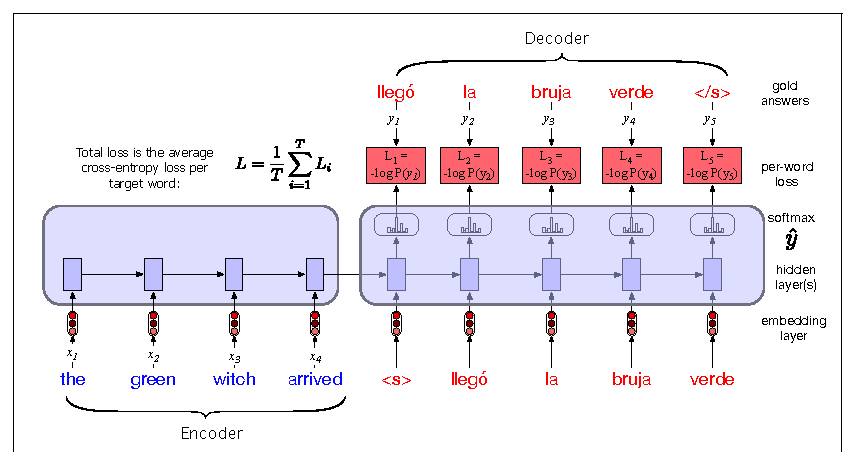
\includegraphics[height=0.56\textheight]{J14_19}
  \end{center}
  \vspace{-0.5em}
  {\tiny\color{mcMuted}
  Training with teacher forcing: the decoder is fed the gold target
  tokens whatever it predicted; at every position the softmax pays the
  cross-entropy $L_i = -\log P(y_i)$ against the gold answer; the total
  loss is the average over the $T$ target words.
  \hfill Jurafsky \& Martin (2026), Fig.~14.19, \S14.7.1.\par}
\end{frame}

\begin{frame}{What teacher forcing leaves out}
  \vspace{-0.3em}
  \begin{propx}[Exposure bias]\label{th:exposure}
    \small
    Under teacher forcing the decoder is trained only on gold prefixes
    $y_{<t}$; at inference it conditions on its own prefixes
    $\hat y_{<t}$, which it never saw during training. A single early
    error moves it to inputs outside the training distribution, and
    errors can compound along the sequence.
  \end{propx}
  \vspace{0.1em}
  {\footnotesize
  \begin{itemize}\itemsep0.22em
    \item Goodfellow's remedy: mix free-running and teacher-forced
          inputs during training; \alert{scheduled sampling} anneals
          from gold to model inputs
    \item The mismatch is what the previous figure hides: the losses are
          paid on gold inputs, and a free-running decoder never sees them
  \end{itemize}}
  \srcline{Goodfellow et al.\ (2016), \S10.2.1; Bengio et al.\ (2015); Ranzato et al.\ (2016).}
\end{frame}

\begin{frame}{Knowing when to stop}
  \vspace{0.05em}
  {\footnotesize
  \begin{itemize}\itemsep0.30em
    \item A sequence model must also decide the \alert{length} $m$. The
          usual way: a special symbol $\eos$ in the vocabulary, emitted
          when the sequence is done and never fed forward
    \item Equivalently, the model defines
          $P(\mathbf{y}_{1:m}) = P(m)\,P(\mathbf{y}_{1:m} \mid m)$ with $P(m)$
          the probability of stopping at $m$; Goodfellow's other options
          are a Bernoulli ``stop'' output at each step or predicting $m$
          up front
    \item The training data are parallel pairs --- sentences aligned
          with their translations --- with $\eos$ appended to every
          target, so the model learns to end where the data end
  \end{itemize}}
  \srcline{Goodfellow et al.\ (2016), \S10.2.3, Eq.~10.34; Jurafsky \& Martin (2026), \S13.2.2.}
\end{frame}

% =====================================================================
\section{The Bottleneck, and Attention}
% =====================================================================

\begin{frame}{Everything through one vector}
  \begin{center}
    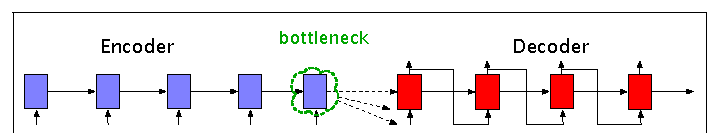
\includegraphics[width=0.80\linewidth]{J14_20}
  \end{center}
  \vspace{-0.5em}
  {\tiny\color{mcMuted}
  The bottleneck: the encoder's last state is the only thing the decoder
  ever sees of the source, and every decoder step draws on it --- $d$
  numbers, however many source tokens went in, written last-word-first
  since the state favours what it read most recently.
  \hfill Jurafsky \& Martin (2026), Fig.~14.20, \S14.8.\par}
\end{frame}


\begin{frame}{Attention, defined}
  \vspace{-0.45em}
  \begin{defx}[Dot-product attention]\label{th:attention}
    \small
    At decoder step $i$, score every encoder state against
    $\mathbf{h}^d_{i-1}$, normalise, and average:
    \[
      \mathrm{score}(\mathbf{h}^d_{i-1}, \mathbf{h}^e_j) = \mathbf{h}^d_{i-1}\cdot\mathbf{h}^e_j, \qquad
      \alpha_{ij} = \frac{\exp \mathrm{score}(\mathbf{h}^d_{i-1}, \mathbf{h}^e_j)}
                         {\sum_k \exp \mathrm{score}(\mathbf{h}^d_{i-1}, \mathbf{h}^e_k)}, \qquad
      \mathbf{c}_i = \sum_{j=1}^{n} \alpha_{ij}\,\mathbf{h}^e_j,
    \]
    and use $\mathbf{c}_i$ in place of $\mathbf{c}$:
    $\mathbf{h}^d_i = g(\hat{\mathbf{y}}_{i-1}, \mathbf{h}^d_{i-1}, \mathbf{c}_i)$.
  \end{defx}
  \vspace{-0.1em}
  {\footnotesize
  \begin{itemize}\itemsep0.16em
    \item Still one vector, but a \alert{different one at each step},
          made from all the encoder states and chosen by the decoder
    \item The dot product needs equal dimensions; the \alert{bilinear}
          score $\mathbf{h}^{d\,\mathsf T}_{i-1}\mathbf{W}_s\mathbf{h}^e_j$ learns
          what to compare and allows different ones
  \end{itemize}}
  \vspace{-0.3em}
  \srcline{Jurafsky \& Martin (2026), Eqs.~14.34--14.37, Figs.~14.21--14.22; Bahdanau et al.\ (2015); Luong et al.\ (2015).}
\end{frame}

\begin{frame}{Attention, drawn: a context per step}
  \begin{center}
    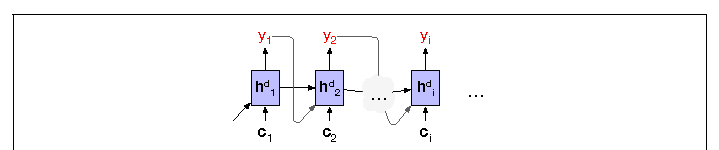
\includegraphics[width=0.62\linewidth]{J14_21}
  \end{center}
  \vspace{-0.5em}
  {\tiny\color{mcMuted}
  The decoder with one change: a different context $\mathbf{c}_i$ enters
  each decoder step $i$, computed from all the encoder states for that
  step.
  \hfill Jurafsky \& Martin (2026), Fig.~14.21, \S14.8.\par}
\end{frame}

\begin{frame}{Attention, drawn: one decoder step in full}
  \begin{center}
    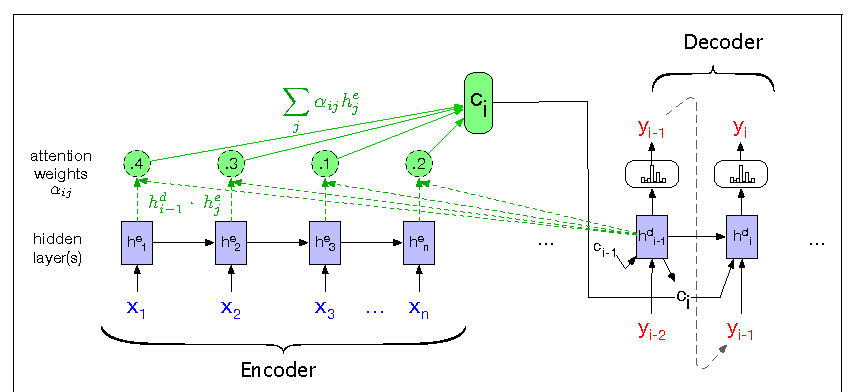
\includegraphics[width=0.86\linewidth]{J14_22}
  \end{center}
  \vspace{-0.5em}
  {\tiny\color{mcMuted}
  Computing $\mathbf{c}_i$: the previous decoder state is scored against
  every encoder state; a softmax turns the scores into the attention
  weights $\alpha_{ij}$; $\mathbf{c}_i$ is the encoder states averaged with
  those weights, and enters decoder step $i$.
  \hfill Jurafsky \& Martin (2026), Fig.~14.22, Eqs.~14.34--14.37.\par}
\end{frame}
\begin{frame}{Where the context can be}
  \vspace{-0.45em}
  \begin{propx}[The context is a convex combination]\label{th:hull}
    \small
    Since $\alpha_{ij} \geq 0$ and $\sum_j \alpha_{ij} = 1$, the context
    $\mathbf{c}_i$ lies in the convex hull of $\{\mathbf{h}^e_1, \dots, \mathbf{h}^e_n\}$;
    the fixed context $\mathbf{c} = \mathbf{h}^e_n$ is one vertex of it, the
    same at every step.
  \end{propx}
  \vspace{0.05em}
  {\footnotesize
  \begin{itemize}\itemsep0.2em
    \item \focus{1}{Proof. A softmax output is a probability vector; an
          average with probability weights is a convex combination.
          \hfill $\square$}
    \item \focus{2}{Attention invents nothing: it picks a point among
          what the encoder computed. The bottleneck was one corner.}
  \end{itemize}}
\end{frame}

\begin{frame}{What attention is, and is not, today}
  \vspace{0.05em}
  {\footnotesize
  \begin{itemize}\itemsep0.30em
    \item Attention here is a \alert{fix to the bottleneck}: the decoder
          reads all the encoder states instead of the last, weighted
          by relevance to where it is
    \item It adds no recurrence and, with the dot product, no
          parameters; with $\mathbf{W}_s$, one matrix
    \item The weights $\alpha_{ij}$ are a by-product worth looking at:
          they say which source tokens produced which target token,
          an alignment nobody labelled
    \item Classes 30--31 will take this one idea, let every token attend
          to every other, and remove the recurrence altogether. Nothing
          in that needs more than Definition~\ref{th:attention}
  \end{itemize}}
  \vspace{0.3em}
  \begin{redhighlight}
    A recurrent encoder--decoder with attention is the last recurrent
    architecture in the course, and the first attention.
  \end{redhighlight}
  \srcline{Jurafsky \& Martin (2026), \S14.8; Bahdanau et al.\ (2015).}
\end{frame}

% =====================================================================
\section{Decoding}
% =====================================================================

\begin{frame}{Choosing the output}
  \vspace{-0.3em}
  \begin{defx}[Greedy and beam decoding]\label{th:beam}
    \small
    The model gives $p(y_t \mid y_{<t}, \mathbf{x})$; decoding must pick one
    $\mathbf{y}$. \alert{Greedy} decoding takes
    $\hat y_t = \arg\max_w p(w \mid \hat y_{<t}, \mathbf{x})$ at each step.
    \alert{Beam search} of width $k$ keeps the $k$ most probable prefixes
    at every step: extend each by every token, score the extensions by
    $\log p(\text{prefix}) + \log p(w \mid \text{prefix}, \mathbf{x})$, and keep
    the $k$ best; a prefix that emits $\eos$ is complete.
  \end{defx}
  \vspace{0.05em}
  {\footnotesize
  \begin{itemize}\itemsep0.22em
    \item The most probable sequence is not the sequence of most
          probable tokens: a locally best token can lead only to bad
          continuations
    \item Exhaustive search over $|V|^m$ sequences is out of the
          question; greedy is $k = 1$; typical $k$ is $5$ to $10$
  \end{itemize}}
  \srcline{Jurafsky \& Martin (2026), \S13.4, Fig.~13.7; Sutskever et al.\ (2014).}
\end{frame}

\begin{frame}{Greedy against beam, on a toy vocabulary}
  \begin{center}
    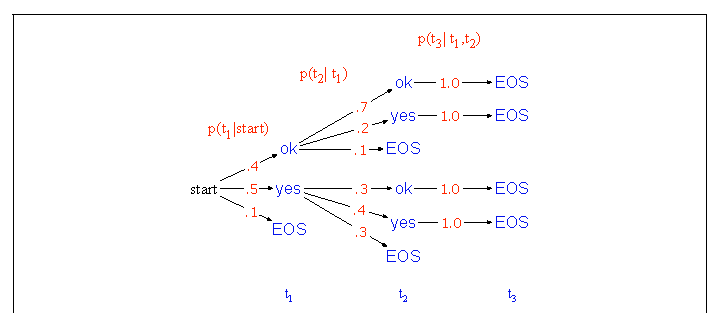
\includegraphics[width=0.80\linewidth]{J13_7}
  \end{center}
  \vspace{-0.5em}
  {\tiny\color{mcMuted}
  A search tree over a toy vocabulary \emph{ok}, \emph{yes}, $\eos$,
  each branch labelled with its probability. Greedy takes \emph{yes} at
  $0.5$ and ends at $0.20$; a beam of width $2$ keeps \emph{ok} and
  \emph{yes}, extends both, and returns \emph{ok ok} $\eos$ at $0.28$: a
  worse first step, a better sentence.
  \hfill Jurafsky \& Martin (2026), Fig.~13.7, \S13.4.\par}
\end{frame}

\begin{frame}{What the beam costs, and what it does not buy}
  \vspace{-0.3em}
  \begin{propx}[Cost and optimality of beam search]\label{th:beamcost}
    \small
    Beam search of width $k$ over sequences of length at most $m$ and
    vocabulary $V$ scores $O(k\,m\,|V|)$ candidates, against $|V|^m$
    for exhaustive search. It is not guaranteed to find the most
    probable sequence: any prefix that falls outside the top $k$ at
    some step is lost, whatever its continuations would have scored.
  \end{propx}
  \vspace{0.05em}
  {\footnotesize
  \begin{itemize}\itemsep0.22em
    \item \focus{1}{Proof of the cost. At each of $m$ steps, each of $k$
          prefixes is extended by each of $|V|$ tokens and the $k$ best
          kept: $k|V|$ scores per step. \hfill $\square$}
    \item \focus{2}{Longer sequences have more factors below one, so raw
          $\log p$ favours short outputs; the standard fix normalises by
          length, $\frac{1}{m}\sum_t \log p(y_t \mid \cdot)$.}
    \item \focus{3}{Minimum Bayes risk decoding picks, from the
          candidates, the one most similar to the rest --- one line,
          and beyond today.}
  \end{itemize}}
  \vspace{-0.3em}
  \srcline{Jurafsky \& Martin (2026), \S13.4, Eq.~13.16, \S13.4.1.}
\end{frame}

% =====================================================================
\section{Putting It Together}
% =====================================================================

\begin{frame}{One model, four settings}
  \vspace{0.2em}
  {\scriptsize
  \renewcommand{\arraystretch}{1.36}
  \begin{tabular}{@{}l@{\hspace{1.0em}}l@{\hspace{1.0em}}l@{\hspace{1.0em}}l@{}}
    & \textbf{context} & \textbf{decoder input} & \textbf{output choice}\\
    language model & $\bos$ only & own previous output & sample or argmax\\
    encoder--decoder & $\mathbf{c} = \mathbf{h}^e_n$, every step & own previous output & greedy or beam\\
    \ldots\ in training & the same & \alert{gold} previous token & none: loss on gold\\
    \ldots\ with attention & $\mathbf{c}_i = \sum_j \alpha_{ij}\mathbf{h}^e_j$ & as above & as above\\
  \end{tabular}}
  \vspace{0.6em}

  \begin{redhighlight}
    Every row is the same three equations of Definition~\ref{th:lm}
    with a different context and a different source of the previous
    token. The recurrent cell $g$ has not been opened; Class 28 opens it.
  \end{redhighlight}
\end{frame}

\begin{frame}{Takeaways}
  \vspace{-0.1em}
  {\scriptsize
  \begin{enumerate}\itemsep0.24em
    \item A sequence-to-sequence problem has an output of its own length
          and order; Class 26's reader cannot write it, but a language
          model can --- given the source first
    \item A recurrent language model is three equations, and generates
          by feeding its own output back (Definition~\ref{th:lm})
    \item Any distribution over sequences factorises token by token; the
          model parameterises the factors (Theorem~\ref{th:chain})
    \item An encoder--decoder is a conditional language model: read the
          source into a context, then generate
          (Definition~\ref{th:encdec}, Proposition~\ref{th:eqs})
    \item Teacher forcing trains it by maximum likelihood, one softmax
          per gold token (Theorem~\ref{th:tf}); it never sees its own
          mistakes (Proposition~\ref{th:exposure})
    \item A fixed context is a bottleneck, and accuracy falls with source
          length; attention gives every step its own context, a convex
          combination of the encoder states
          (Definition~\ref{th:attention}, Proposition~\ref{th:hull})
    \item Greedy decoding is not the most probable sequence; beam search
          is closer at $O(km|V|)$ (Definition~\ref{th:beam},
          Proposition~\ref{th:beamcost})
  \end{enumerate}}
  \vspace{-0.2em}
  \bridge{Class 28 opens the cell $g$: why a simple RNN forgets, and
  what an LSTM's gates change.}
\end{frame}

\begin{frame}[allowframebreaks]{References}
  \vspace{0.3em}
  {\scriptsize
  \begin{enumerate}\itemsep0.30em
    \item D.\ Jurafsky \& J.\ H.\ Martin, \emph{Speech and Language
          Processing}, 3rd ed.\ draft, August 2026. Ch.~14 \S14.2
          (Eqs.~14.4--14.9, Fig.~14.5), \S14.3.3 (Fig.~14.9), \S14.7
          (Eqs.~14.28--14.33, Figs.~14.16--14.19), \S14.8
          (Eqs.~14.34--14.37, Figs.~14.20--14.22); Ch.~13 \S13.2, \S13.4
          (Fig.~13.7). The course plan's ``Chapter 13'' is this chapter
          in the earlier draft.
    \item I.\ Goodfellow, Y.\ Bengio \& A.\ Courville, \emph{Deep
          Learning}, MIT Press, 2016. \S10.2.1 (Eqs.~10.15--10.16,
          Figs.~10.4, 10.6), \S10.2.3 (Eq.~10.34), \S10.2.4 (Eq.~10.35,
          Figs.~10.9--10.10), \S10.4 (Fig.~10.12).
    \item K.\ Cho et al., ``Learning phrase representations using RNN
          encoder--decoder for statistical machine translation'',
          EMNLP 2014.
    \item I.\ Sutskever, O.\ Vinyals \& Q.\ V.\ Le, ``Sequence to sequence
          learning with neural networks'', NeurIPS 2014.
    \item D.\ Bahdanau, K.\ Cho \& Y.\ Bengio, ``Neural machine
          translation by jointly learning to align and translate'',
          ICLR 2015.
    \item M.-T.\ Luong, H.\ Pham \& C.\ D.\ Manning, ``Effective
          approaches to attention-based neural machine translation'',
          EMNLP 2015.
    \item R.\ J.\ Williams \& D.\ Zipser, ``A learning algorithm for
          continually running fully recurrent neural networks'',
          \emph{Neural Computation} 1(2), 1989.
    \item S.\ Bengio, O.\ Vinyals, N.\ Jaitly \& N.\ Shazeer, ``Scheduled
          sampling for sequence prediction with recurrent neural
          networks'', NeurIPS 2015.
    \item M.\ Ranzato, S.\ Chopra, M.\ Auli \& W.\ Zaremba, ``Sequence
          level training with recurrent neural networks'', ICLR 2016.
    \item T.\ Mikolov et al., ``Recurrent neural network based language
          model'', Interspeech 2010.
    \item C.\ E.\ Shannon, ``Prediction and entropy of printed English'',
          \emph{Bell System Technical Journal} 30, 1951.
  \end{enumerate}}
\end{frame}

\begin{frame}[standout]
  Questions?
\end{frame}

\end{document}
